\documentclass[11pt, oneside]{article}
\usepackage{titling, hyperref, geometry, amsmath, amssymb, algorithm, graphicx, textcomp, subcaption, cancel, float}
\usepackage[noend]{algpseudocode}
\usepackage[cache=false]{minted}
\geometry{a4paper}

\hypersetup{
    colorlinks=true,
    urlcolor=cyan
}

\newcommand{\emphasis}[1]{\textcolor{blue}{\textbf{\textit{#1}}}}
\newcommand{\smallemphasis}[1]{\textbf{\textit{#1}}}

\title{Flow}
\author{Udbhav Muthakana \\ Edited by: Stephen Huan}

\begin{document}
\maketitle

\section{Definition}
Let \( G \) be a directed graph (no self-loops) with nonnegative edge weights, henceforth known as ``capacities''. Out of the set of vertices \( V \), we define one vertex to be our source, \( s \), and another to be our sink, \( t \). The \smallemphasis{flow} function \(f(u, v) \) through \( G \) and the capacity function \( c(u, v) \) satisfy the following requirements:

\begin{enumerate}
   \item \( f(u, v) \leq c(u, v) \) for all \( u, v \in V \)
   \item \( \sum_{v \in V} f(v, u) = \sum_{v \in V} f(u, v) \) for all \( u, v \in V - \{s, t\} \)
\end{enumerate}

Condition 1 means the flow through an edge cannot exceed the capacity of that edge.

Condition 2 is a little harder to understand, but means the flow into a vertex must equal the flow out of a vertex (excluding, of course, the source and the sink).

\begin{figure}[h!]
\centering
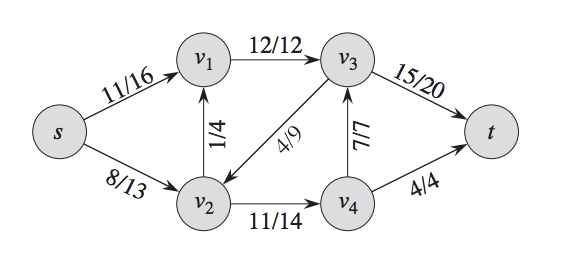
\includegraphics[scale=1]{flowdiagram}
\caption{A flow network - edges are labeled with \( f/c \)}
\end{figure}

The \smallemphasis{maximum flow problem} is then defined as finding the maximum possible flow \( f \) through \( G \).

\newpage
\subsection{Useful Transformations}

Our definition of a flow network is rather restrictive, but luckily there are several ways to transform networks into proper flow networks without changing their maximum flows.

First, edges connecting a vertex to itself can safely be ignored, as they do not add any flow to the network

Second, we often see networks with multiple sources and sinks. To remedy this, we create a ``supersource'' and a ``supersink'' that connect to every source and every sink respectively. The capacities for their connections are set to infinity.

\begin{figure}[H]
\centering
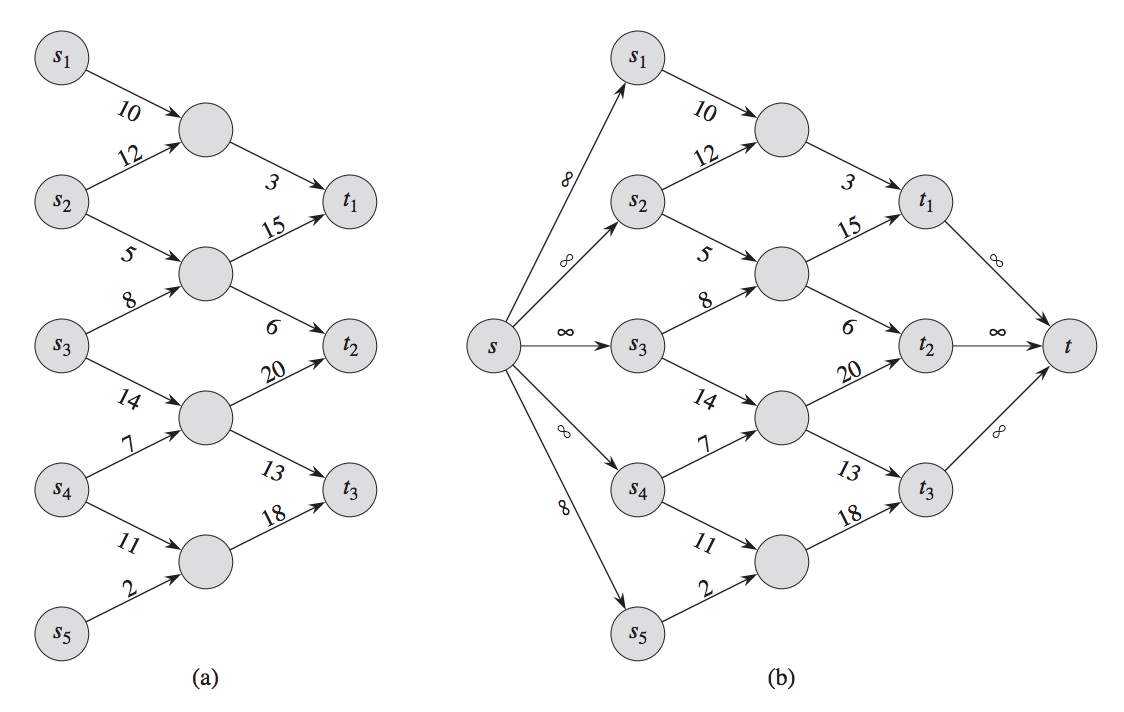
\includegraphics[scale=0.4]{supersourcesink}
\caption{Transformation of a network with multiple sources and sinks}
\end{figure}

Third, we are occasionally given networks with vertex capacities as well as edge capacities. The relevant transformation involves splitting each vertex \( v \) with capacity \( c \) into \( v_1 \) and \( v_2 \), which are connected by an edge of capacity \( c \). We then connect \( v \)'s incoming edge to \( v_1 \) and the outcoming edge to \( v_2 \).


Finally, if networks with antiparallel edges (that is, edges \( (u, v) \) and \( (v, u) \)) bother you, they are easily transformed. For each pair of antiparallel edges, we arbitrarily choose one edge and split it into two edges of equal capacity, inserting a new vertex (\( v' \)) between them. The algorithms we discuss do not require the input network to have no antiparallel edges - this transformation is purely for human comfort.

\begin{figure}[H]
\centering
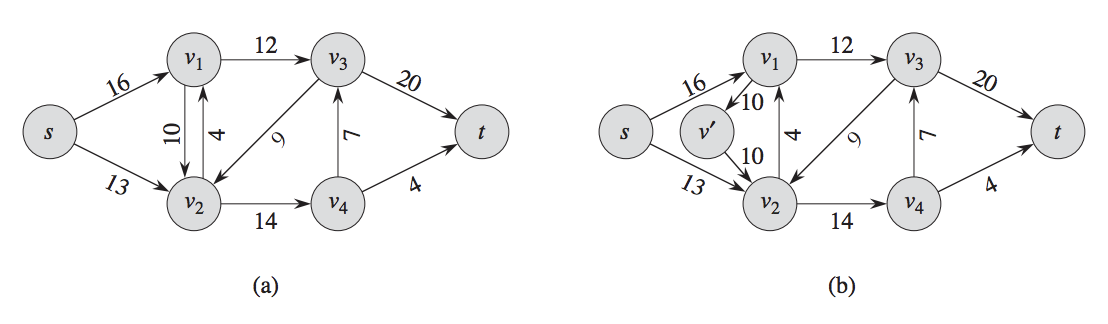
\includegraphics[scale=0.75]{antiparallel}
\caption{Transformation of a network with antiparallel edges}
\end{figure}

\newpage
\subsection{Residual Networks}

The \smallemphasis{residual network} \( G_f \) is a flow network that represents the changes we can make to \( G \). To construct \( G_f \), we iterate over the edges of \( G \) and obey the following rules:

\begin{enumerate}
   \item If \( f(u, v) < c(u, v) \), we add a new edge \( (u_f, v_f) \) with capacity \( c(u, v) - f(u, v) \)

   \item If \( f(u, v) > 0 \), we add a new edge \( (v_f, u_f) \) with capacity \( f(u, v) \)
\end{enumerate}

For example, consider the following flow network \textbf{(a)} and its residual network \textbf{(b)}

\begin{figure}[h]
\centering
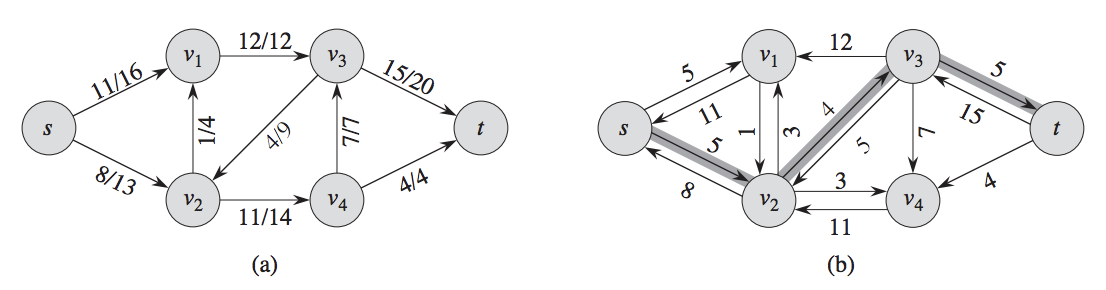
\includegraphics[scale=0.75]{residualnetwork}
\caption{A graph and its residual network with the augmenting path highlighted}
\end{figure}

The edge \( (s, v_1) \) in the original graph has \( f = 11 \) and \( c = 16 \), so we can increase its flow by \( 16 - 11 = 5 \). Thus, in the residual graph, \( c_f(s, v_1) = 5 \). We can also decrease the flow by \( f(s, v_1) \), so we create an antiparallel edge: \( c_f(v_1, s) = 11 \).


The \smallemphasis{augmenting path} is a simple (no cycles) path between \( s \) and \( t \) on the residual graph. Since each \( c_f(u, v) \) on the residual graph represents the amount we can increase the flow on \( (u, v) \), we can increase the flow of every edge along the augmenting path by the minimum \( c_f \) along the path.

More formally, the \smallemphasis{residual capacity} of an augmenting path \( p \) is
\begin{center}
\[ r_c = \min_{(u, v) \in p} \ c_f(u, v) \]
\end{center}

The presence of an augmenting path means we can improve the flow of the network by at least the residual capacity.

\subsection{Cuts}

A \smallemphasis{cut} of a flow network is a split of \( V \) into two vertex sets, \( S \) and \( T \) such that \( S \) contains the source and \( T \) contains the sink.

The capacity of a cut is defined as the sum of the capacities of the edges that connect \( S \) to \( T \). Note that we do \textbf{not} include edges in the reverse direction. More formally, the cut capacity is
\[ \sum_{u \in S} \sum_{v \in T} c(u, v) \]

\newpage

The \smallemphasis{max-flow min-cut} theorem states that
\begin{enumerate}
   \item The maximum flow of \( G \) is equal to the capacity of the minimum cut of \( G \)
   \item When the flow is maximum, there is no augmenting path in \( G_f \)
\end{enumerate}

\section{Algorithms}

\subsection{Ford-Fulkerson}

Ford-Fulkerson is a popular tool for max-flow problems. It is more of a method than an algorithm, providing a framework that many algorithms with different complexities draw from.

The method continually finds the residual network \( G_f \) and looks for an augmenting path. If found, it increases the flow along every edge of the path by the residual capacity. The logic stems from the second implication of the max-flow min-cut theorem: once an augmenting path no longer exists, flow is maximized. Since each iteration of the augmenting path provides us with a flow gain of at least 1 (assuming integral flow values), the method is guaranteed to converge to the maximum flow.

\begin{algorithm}
  \begin{algorithmic}[h!]
    \Procedure{Ford-Fulkerson}{$G$, $s$, $t$}
      \For{each edge (u, v) in G.E}
          \State set flow through (u, v) to 0
      \EndFor
      \While{augmenting path $p$ in $G_f$ exists}
         \State $r_c = \min(c_f(u, v)$ for $u, v$ in $p)$
         \For{each edge $(u, v)$ in G.E}
            \State $f(u, v) = f(u, v) + r_c$
            \State $f(v, u) = f(v, u) - r_c$
         \EndFor
      \EndWhile
    \EndProcedure
  \end{algorithmic}
\end{algorithm}

Note that the method does not specify \textbf{how} we find an augmenting path. Our choice here is important to ensure our algorithm runs reasonably fast.
\subsection{Edmonds-Karp}

\href{https://gist.github.com/stephen-huan/d660e04476f06695663401d0ac01a27a#flow}{Edmonds-Karp} is an implementation of Ford-Fulkerson that uses a BFS to find the augmenting path. BFS will provide an augmenting path with the shortest length, but why does this guarantee convergence to the maximal flow?

For every augmenting path in a residual network, one \smallemphasis{critical edge} has the lowest capacity and thus determines the path's residual capacity. Once we augment flow along the path, the critical edge is filled and will not appear in future residual graphs. However, it may appear again as a ``reduction'' edge (i.e to represent decreasing flow through that edge). This will happen at most \( V/2 \) times per critical edge, so the number of augmentations is bounded by \( O(VE) \).

Since each augmentation takes \( O(E) \) in Ford-Fulkerson, our final complexity for Edmonds-Karp is \( O(VE^2)\). This is sufficient for most flow problems and is simple to code (sample implementation linked above), but neither asymptotically nor practically optimal. A common technique that yields asymptotically and practically faster times is called ``push-relabel''.


\section{Push-relabel}

Push-relabel, like Ford-Fulkerson, is method that many algorithms draw from. During the operation of push-relabel algorithms, flow conservation is not strictly maintained. Instead, we maintain a \smallemphasis{preflow} that allows vertices to have more flow in than flow out. The delta between flow in and flow out (which must be \( \geq \) 0) is called \smallemphasis{excess flow}.

There are two main operations suggested by the name: \smallemphasis{push}ing preflow and \smallemphasis{relabel}ing a vertex. Before we discuss those, however, we must define one more concept: the \smallemphasis{height} of a vertex. Each vertex has a height that will change with relabel operations. Since the sink has a height of 0, the operation of the push-relabel algorithm resembles pushing flow down a hill.

Before commencing any push or relabel operations, we first set the preflow from the source:

\begin{algorithm}
  \begin{algorithmic}[h!]
    \Procedure{Set-Preflow}{$G$, $s$}
      \For{each vertex v in G.V}
         \State $v.h = 0$
         \State $v.e = 0$
      \EndFor
      \For{each edge (u, v) in G.E}
         \State $(u, v).f = 0$
      \EndFor
      \State $s.h = |G.V|$
      \For{each vertex v adjacent to s}
         \State $(s, v).f = c(s, v)$
         \State $v.e = c(s, v)$
         \State $s.e -= c(s, v)$
      \EndFor
    \EndProcedure
  \end{algorithmic}
\end{algorithm}

The first and second for loops initialize flows, excesses, and heights to 0. The three statements in the last for loop push the maximum amount of flow from the source, set the excess flow of the vertices proximate to the source, and set the excess of the source to be negative.

The push operation on an overflowing vertex (excess flow \( > \) 0) \( u \) pushes as much excess flow as possible to a neighbor \( v \). The push operation is called if and only if \(u.h - v.h = 1 \). That is, flow is only pushed downhill and between vertices with a height differential of 1.

The relabel operation is called when a vertex \( u \) with excess flow \( > 0 \) has no neighbors with the proper height. We increase the height of \( u \) to \( 1 + v.h \), where \( v \) is the neighbor of minimum height.

The actual push-relabel algorithm is rather simple:
\newpage
\begin{algorithm}
  \begin{algorithmic}[h!]
    \Procedure{Push-Relabel}{$G$, $s$}
      \State Set-Preflow(G, s)
      \While{node $u$ with overflow exists}
         \If{can push}
            \State Push($G$, $u$)
         \Else
            \State Relabel($G$, $u$)
         \EndIf
      \EndWhile
    \EndProcedure
  \end{algorithmic}
\end{algorithm}


The variations among push-relabel algorithms mostly come from unique ways of choosing which node to process next. The generic push-relabel algorithm has complexity \( O(V^2 E) \), an improvement over Edmonds-Karp.


\section{Bipartite Matching}

\subsection{Bipartite graphs}

Bipartite matching problems are the most common use of flow algorithms in competitive programming settings. A \smallemphasis{bipartite graph} is a graph whose vertices are split into two disjoint sets, such that every edge bridges the sets. The sets are usually visualized vertically, as shown in Figure 5. The \smallemphasis{maximum bipartite matching} is the subset of edges of maximum size such that no two edges share an endpoint.

\begin{figure}[H]
\centering
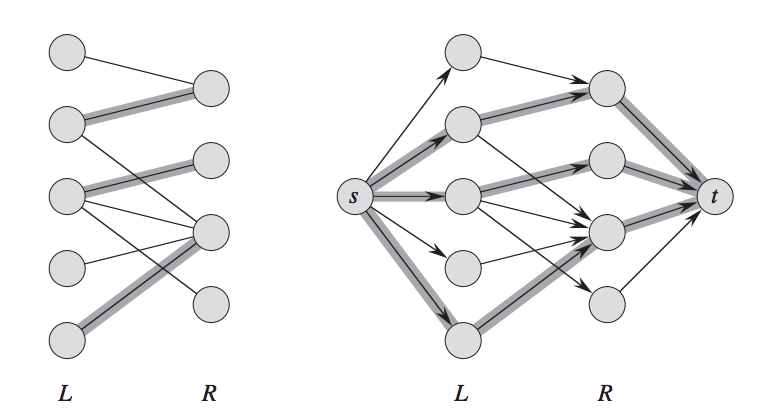
\includegraphics[scale=0.75]{maximum-bipartite-matching}
\caption{A bipartite graph and its flow network with the maximum matching highlighted}
\end{figure}

The maximum bipartite matching problem can be solved with the previously discussed flow algorithms as follows: perform the transformation discussed in section 1.1, creating a supersource and supersink (shown in Figure 5). Then, treating the edges between L and R as directed toward R, we assign every edge a capacity of 1 and run our flow algorithm. The maximum flow is equivalent to the size of the maximum bipartite matching.

\subsection{Hopcroft-Karp}

The Hopcroft-Karp algorithm is a faster way to solve the maximum bipartite matching problem. While Edmonds-Karp runs in \( O(VE^2)\), Hopcroft-Karp runs in \( O(E\sqrt{V})\). As this speedup is rarely necessary in competitive programming, the implementation is outside the scope of this lecture. However, many resources exist online should you wish to implement it yourself.

\newpage
\section{Sample Problems}

\begin{enumerate}
   \item \href{https://www.spoj.com/problems/MTOTALF/}{SPOJ Total Flow}: Given a network of \( N \) (\( 1 \leq N \leq 700 \)) water pipes that connect a well to the barn, Farmer John wishes to calculate the net flow capacity through the pipes.

   Solution: A straightforward Edmonds-Karp implementation passes. Note that to construct a proper flow graph, you need to combine the capacities of multiple pipes between the same vertices.

   \item USACO Drainage Ditches (Training section 4.2) \href{http://poj.org/problem?id=1273}{POJ link}: Same as above with (\( 0 \leq N \leq 200 \))

   Solution: Another Edmonds-Karp problem.

   \item \href{https://www.spoj.com/problems/POTHOLE/}{SPOJ Potholers}: Several speleologists organize a training session in a mountain with \( N \) (\( 0 \leq N \leq 200 \)) chambers that are semi-connected by corridors. During the training, each speleologist explores a route from the top chamber, \( T \), to the bottom chamber, \( B \). The speleologists may only move down, i.e. the level of every consecutive chamber on a route must be lower then the previous one. Each speleologist has to start from \( T \) through a different corridor, and each of them must enter \( B \) using different corridor. The remaining corridors may be traversed by more than one speleologist. How many speleologists can train simultaneously?

   Solution: We are given the graph, but need to determine corridor capacities. To satisfy the ``one-per-corridor'' condition, the capacity of any corridor that links to either \( T \) or \( B \) must be one. The intermediate corridors should have infinite (or arbitrarily large) capacities, and then we can just run Edmonds-Karp.

   Sidenote: the input format for this problem is rather convoluted, so you should check that first if you're getting wrong answers.

   \item \href{http://www.usaco.org/index.php?page=viewproblem2&cpid=93}{USACO Cow Steeplechase (November 2011)}: Given a list of horizontal and vertical line segments, find the maximum number of segments such
   that no two intersect. No segments overlap each other.

   Solution: We can represent the problem as a bipartite graph with horizontal lines as vertices in one set and vertical lines in the other. An edge represents an intersection between two lines. We can simply structure the graph as a flow problem and run any maximum flow algorithm. However, we aren't done, as we've only found the minimum cut (in this case, the minimum node cover). It can be proven that the complement of the minimum node cover is the maximum independent set in any graph. Thus, the answer is the total number of nodes minus the maximum flow value we computed.

   \item \href{http://poj.org/problem?id=3041}{USACO Asteroids (November 2005)}: A rectangular grid has some marked cells (asteroids). Zapping a row destroys all asteroids in the row. Zapping a column destroys all the asteroids in the column. Find the minimum number of zaps to destroy the asteroids.

   Solution: Similarly to Cow Steeplechase, we represent the problem as a bipartite graph with rows as vertices in one set and columns in the other. A row is connected to a column if there exists an asteroid in the intersection of that row and column. All edges have a weight of 1. The minimum cut of the network is guaranteed to remove all asteroids, as there are then no paths from source to sink. The rules don't allow us to remove individual asteroids, but we can always achieve the same effect with the removal of some edge from the supersource to a row or from a column to the supersink. Thus, the answer is simply the minimum cut, or maximum flow, of the network.

\end{enumerate}

\section{Past Lectures}

\begin{enumerate}
   \item \href{https://activities.tjhsst.edu/sct/lectures/1516/SCT_Maximum_Flow.pdf}{(Broken) ``Maximum Flow'' (Samuel Hsiang, 2015)}
   \item \href{https://activities.tjhsst.edu/sct/lectures/1112/networkflow.pdf}{``Introduction to Network Flow'' (Alex Chen, 2012)}
   \item \href{https://activities.tjhsst.edu/sct/lectures/0910/network_flow.pdf}{``Network Flow'' (Andre Kessler, 2009)}
   \item \href{https://activities.tjhsst.edu/sct/lectures/0607/netflownew.pdf}{``Network Flow'' (Tom Morgan, 2006)}
   \item \href{https://activities.tjhsst.edu/sct/lectures/0304/netflow.pdf}{``Network Flow'' (No author, 2004)}
\end{enumerate}

\section{Works Cited}

\begin{enumerate}
   \item \href{https://mitpress.mit.edu/books/introduction-algorithms-third-edition}{\textit{Introduction to Algorithms}} (also known as CLRS)
\end{enumerate}

\end{document}
